\section{Introduction}
\label{sec:intro}

Entity resolution (ER) is the task of mapping mentions of entities in
text to corresponding records in a knowledge base (KB)
\cite{BunescuP06,Cucerzan07,KulkarniSRC09,Dredze2010,Hoffart2011,Hachey2013130}.
%with numerous applications
%\cite{Gabrilovich2007,Lin2012,Kwiatkowski2011,finin2009Coreference,mayfield2009cross}.
%Key applications are to information extraction and grounded semantic
%parsing. %text classification~\cite{Gabrilovich2007}, information
%extraction~\cite{Lin2012} and grounded semantic
%parsing~\cite{Kwiatkowski2011}.  It can also provide a valuable
%signal to other language-processing tasks, including part-of-speech
%tagging, parsing, and coreference
%resolution~\cite{finin2009Coreference,mayfield2009cross}.  Entity
%resolution
ER is a challenging problem, because mentions are often ambiguous on
their own, and can only be resolved given appropriate context.  For
example, the mention \qtext{Beirut} may refer to the capital of
Lebanon, the band from New Mexico, or a drinking game
(Figure~\ref{fig:ereg}.)
% Names may also refer to entities that are not in the KB, a problem
% known as \emph{{\NIL} detection}.
ER can improve text classification \cite{Gabrilovich2007}, information
extraction \cite{Lin2012}, coreference resolution
\cite{finin2009Coreference,mayfield2009cross} and other
language-processing tasks.
%Kwiatkowski2011groundedsemparsing

Most ER systems consist of a \emph{mention model}, a \emph{context
  model}, and a \emph{coherence
  model}~\cite{Milne2008,Cucerzan07,Ratinov11,Hoffart2011,Hachey2013130}
The mention model associates each entity with its possible textual
representations, also called aliases or surface forms.  The context
model helps resolve an ambiguous mention using textual features
extracted from the surrounding context, such as the enclosing sentence
and salient noun phrases in the document. The coherence model, which
is our focus in this work, encourages all mentions to resolve to
entities that are related to each other.  Relations may be established
via the KB, Web links, embeddings, or other resources.

Coherence models often define an objective function that includes
local and pairwise candidate scores, where the pairwise scores
correspond to some notion of coherence or relation
strength\footnote{An exception to this framework are topic models in
  which a topic may generate both entities and words, e.g.,
  \cite{kataria2011,HanS12,houlsby2014scalable}.}. Finding an entity
labeling that maximizes the objective is usually intractable and
tackled via various approximations, which we discuss in more detail in
Section~\ref{sec:related}.

\begin{figure*}[t]
\centering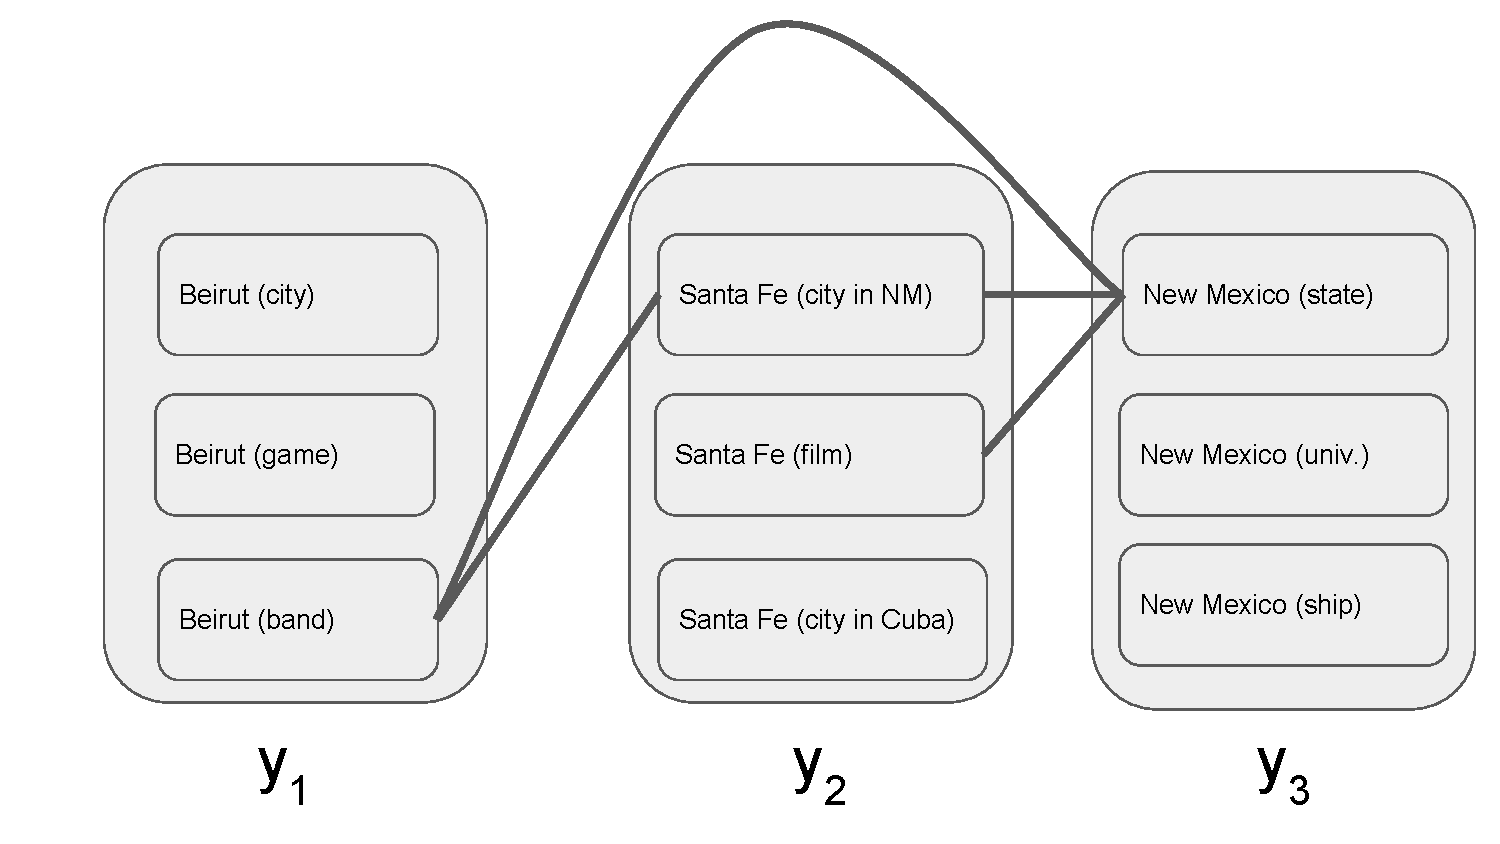
\includegraphics[width=0.5\linewidth]{beirut.pdf}
\caption{Illustration of the ER problem for three mentions
  ``Beirut'', ``New Mexico'' and ``Santa Fe''. Each mention has three
  possible disambiguations. The links indicate disambiguations that
  have wikipedia links between their respective pages.
\todo{show sample text?}}
\label{fig:ereg}
\end{figure*}

All-pairs coherence objectives aggregate over salient, well-connected
entities and less prominent entities that are not so well-connected.
In effect, all-pairs objectives seek evidence in favor of a candidate
entity from \emph{all} other mentions in the document, evidence that
may simply not exist for non-salient entities.  However, valuable
support in favor of a candidate entity may be provided by a small
number of entities chosen for other mentions.  Thus, all-pairs
objectives risk losing these delicate signals.  Our primary goal is to
fix this problem.

In this work, we introduce a novel coherence model with a multi-focal
attention mechanism. In our model, the coherence score for each
candidate entity depends on a small set of mentions it attends to,
rather than all mentions in the document. Attention has recently been
used with considerable empirical success in tasks such as translation
\cite{bahdanau2014neural} and image caption generation
\cite{xu2015show}. We argue that attention is also desirable for
collective ER due to the discussed imbalance in the number of
relations for different entities.

Our model relies on a novel smooth version of the multi-focus
attention function, which generalizes the single-focus softmax
function. We use a simple and efficient inference procedure, and show
how the model parameters can be learned from data.

We augment a competitive local context model (which does not use a
coherence model) similar to \cite{Lazic2015} with our new coherence
formulations.  We see performance improvements on three benchmarks.
On the CoNLL 2003 dataset \cite{Hoffart2011}, we see a relative
reduction in error (RRIE) of \todo{FILL\%}.  On the TAC KBP 2010--2012
datasets, we get a RRIE of in-KG entities around \todo{FILL\%}.

Our contributions thus consist of defining a novel multi-focal
attention based model, where inference is efficient, and applying it
successfully to an entity resolution system.  Our model can be applied
to other structured prediction problems in NLP.  \todo{Drop or elaborate}

%Our premise is that this may also hold for entity relations:
%aggregating support for an entity label over the whole document may
%dilute the evidence for non-salient entities. We explore two new
%approaches to coherence that focus on a \emph{limited number} of
%relations for each candidate, rather than relations to all other
%entities.
%\begin{figure*}[!ht]
\begin{tikzpicture}[node distance=1.5cm,>=stealth',bend angle=35,auto]
  \tikzstyle{candidate}=[rectangle,dashed,rounded corners=2mm,thick,draw=black,fill=white,minimum size=6mm]
  \tikzstyle{selected} = [rectangle,rounded corners=2mm,thick,draw=black,fill=gray!10,minimum size=6mm]
  \tikzstyle{mention}=[rectangle,thick,draw=black!75,
  			  fill=black!10,minimum size=6mm]
  \tikzstyle{every label}=[black]

 \begin{scope}
    % First mention.
   % \node [mention] (m1){\qtext{Beirut}};
   % \node [candidate] (c11) [label=above:0.5] {Beirut, Lebanon};
   \node [candidate] (c11) {Beirut, Lebanon};
    \node [candidate] (c12) [below of=c11]  {Beirut (game)};
    \node [selected] (c13)  [below of=c12] {Beirut (band)};

   % Second mention.
   % \node [mention] [right=3cm of m1](m2){\qtext{Santa Fe}};
    \node [selected] (c21) [right=2cm of c11] {Santa Fe, New Mexico};
        \node [candidate] (c22) [below of=c21]  {Santa Fe (1951 Western)};
    \node [candidate] (c23)  [below of=c22] {Santa Fe (Beirut song)};

      
     % Third mention.
   % \node [mention] [right=3cm of m2](m3){\qtext{New Mexico}};
    \node [selected] (c31) [right=2cm of c21] {New Mexico (state)};
    \node [candidate] (c32)  [below of=c31] {Univ. New Mexico};
 
      
   %\path (c13) edge [post,line width=2pt] node[above]{0.5} (c21);
   \path (c13) edge [post,line width=2pt] (c21);
   \path (c13) edge [post,dashed,line width=2pt] (c23);
   \path (c31) edge [post,line width=2pt] (c21);
   \path (c21) edge [post,line width=2pt,bend right] (c31);
  \end{scope}
\end{tikzpicture}
\caption{Example coherency graph for mentions $\qtext{Beirut}$, $\qtext{Santa Fe}$ and $\qtext{New Mexico}$. Solid lines indicate a valid solution subgraph, where each selected candidate has at most one outgoing edge to another candidate. TODO: better example?}
\label{fig:graph}
\end{figure*}


%  Accordingly, we propose to choose the label for each mention based on the best support from a \emph{limited number} of other mentions.  In other words,  each mention is labeled by (tractable) inference in a star graph, but one where most edges are (dynamically) ignored.

\comment{
\subsection{Our contributions}
\label{sec:intro:our}


In the first approach, which we name \emph{single link}, we formulate inference as finding the highest-weight subgraph in which each candidate has a directed edge to \emph{at most} one other candidate. This can roughly be seen as maximizing over relations as opposed to averaging. In this model we perform inference using max-sum belief propagation \cite{Kschischang2001}.

%; however, it is slightly more computationally involved since an edge between two entities is allowed only if the corresponding mentions resolve to them. 
%We specify the objective and constraints using binary edge-indicator variables, and find the maximum-a-posteriori solution using the max-sum algorithm \cite{Kschischang2001}. 
Our

In the second \emph{attention} model, we allow each mention to have up to $K$ relations to other mentions. In this case, inference is tractable, and we also learn mention and edge scores from a small set of simple features.   %In other words,  each mention is labeled by (tractable) inference in a star graph, but one where most edges are (dynamically) ignored.

We use these coherence models to re-rank candidates generated by Plato \cite{Lazic2015}, a recent entity resolution system that has highly competitive performance and does not include a coherence component. This leads to performance improvements on three benchmarks, and yields new state-of-the-art results on the TAC KBP 2011 and 2012 datasets.
}


\secref{sec:notation} introduces notation.
\secref{sec:attention} presents the new multi-focus attention
model.  \secref{sec:maxsum} discusses a baseline model with
single focus.  \secref{sec:related} reviews related work.
\secref{sec:expt} presents experimental results.



%%% Local Variables: ***
%%% mode:latex ***
%%% TeX-master: "main.tex"  ***
%%% tex-main-file: "main.tex"  ***
%%% End: ***
